\documentclass{article}
\usepackage[utf8]{inputenc}
\usepackage[english,russian]{babel}
\usepackage{graphics}
\usepackage{amsmath}
\usepackage{indentfirst}
\usepackage{misccorr}
\usepackage{amsmath}
\usepackage{graphicx}
\graphicspath{{./pic/}}

\begin{document}





\section{1}
Постройте график функции
\begin{equation*}
y = 
 \begin{cases}
   x^2-4x+5 \text{, если } x \geq 1 \\
   x+1 \text{, если } x<1
 \end{cases}
\end{equation*}
и определите, при каких значениях $m$ прямая $y = m$ имеет с графиком ровно две общие точки.

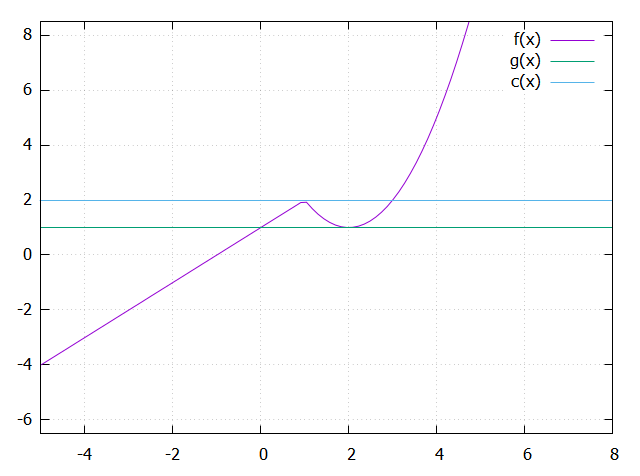
\includegraphics [scale=0.5]{plot.png}

1) $x=1$, $y=1+1=2$, т.е при $m=2$ ровно 2 общие точки.

2) $x^2-4x+5$,
$y_0 = \frac{-D}{4a}=1$, т.е при $m=1$ ровно 2 общие точки.

Ответ: При $m=1$, $m=2$

\section{2}

	Постройте график функции\newline
	$$
		y =
		\begin{cases}
			-x^2, |x| \leq 1, \\
			-\frac{1}{x}, |x| > 1.
		\end{cases}
	$$
	\newline и найдите при каких $c$ данный график и график $ y = c $ имеют
	ровно одну общую точку.
	\newline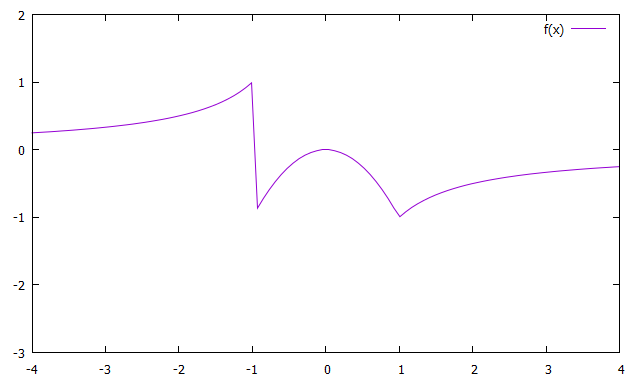
\includegraphics[scale=0.4]{kostya_1.png} \newline
	Исследование:
	\newline\space При $c \in \left[ 1; +\infty \right)$ графики 
	$ y = c $ и данный график имеют 0 общих точек;
	\newline\space При $c \in \left[ 0; 1 \right)$ графики $ y = c $
	и данный график имеют 1 общую точку;
	\newline\space При $c \in \left( -1; 0 \right)$ графики $ y = c $
	и данный график имеют 3 общие точки;
	\newline\space При $c = -1$ графики $ y = c $
	и данный график имеют 2 общие точки;
	\newline\space При $c \in \left( -\infty; -1 \right)$ графики 
	$ y = c $ и данный график имеют 0 общих точек;
	\newline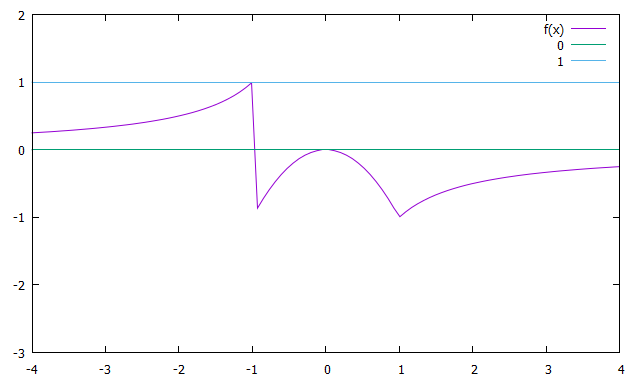
\includegraphics[scale=0.4]{kostya_2.png}
	\newline Ответ: $ c \in \left[ 0; 1 \right) $.

	\section{3}
  
  	Постройте график функции\\
	\begin{equation*}
	y(x) = 
	\begin{cases}
	\frac{5}{x} &\text{если $x < -1$}\\
	-x^2+4x &\text{если $x \ge -1$}\\
	\end{cases}
	\end{equation*}
	и определите, при каких значениях c  прямая {$y=c$}   будет пересекать построенный график в трёх точках.\\
	\graphicspath{{Pictures/}}
	\DeclareGraphicsExtensions{.pdf,.png,.jpg}
	\begin{figure}[hb]
		\begin{center}
			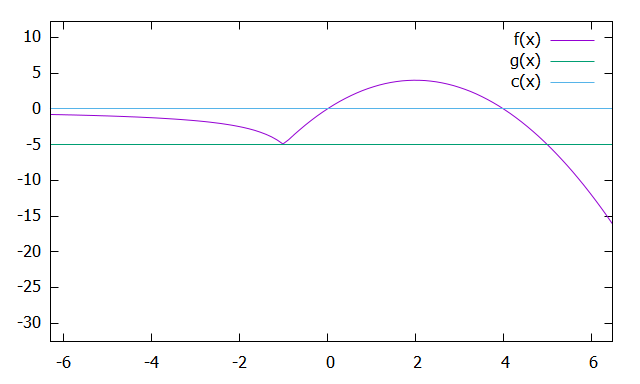
\includegraphics[scale=0.5]{Graphic}
		\end{center}
	\end{figure}
	\\
	\\
	1) При {$c<-5$} график  {$y=c$} будет пересекать график f(x) только в одной точке\\
	2) При {$c \geq 0$}  график  {$y=c$} будет пересекать график f(x) в одной точке, в двух точках или не будет пересекать вовсе\\
	3)При {$c \in [-5;0)$} график  {$y=c$} будет пересекать график f(x) только в трёх точках\\
	Ответ: {$c \in [-5;0)$}
  
\end{document}

